%
%	Presentaci\'on CNF 2018
%
\documentclass[10pt]{beamer}
\usepackage[spanish]{babel}					% En español
\usetheme[secheader]{PaloAlto}				% Warsaw, Madrid, PaloAlto, Ilmenau, 
\usecolortheme[RGB={37,40,80}]{structure}	% Dresden, Boadilla, Goettingen
\usepackage{amssymb,amsfonts,amsmath,amsthm,mathrsfs,braket}  
\usepackage{graphicx,multirow,color,textpos,epstopdf,hyperref}
\setbeamerfont{caption}{series=\normalfont,size=\fontsize{6}{8}}
\usefonttheme{serif}
\makeatletter
\beamer@headheight=1.8\baselineskip	        % Alto de cabecera, default 2.5    
\makeatother
				
%%%%%%%%%%%%%%%%%%%%%%%%%%%%%%%%%%%%%%%%%%%%%%%%%%%%%%%%%%%%%%%%%%%%%%%%%%%%%%%%%

\title[$N^*$ and $\Delta^*$ poles]
{Regge phenomenology of the $N^*$ and $\Delta^*$ poles}
\author[J. Silva C. Fern\'andez]{Jorge Antonio Silva-Castro y  
								C\'esar Fern\'andez-Ram\'irez}
\institute[ICN-UNAM]{
	Instituto de Ciencias Nucleares, Universidad Nacional Aut\'onoma de M\'exico
   \\PAPIIT-DGAPA (UNAM) No. IA101717\\CONACYT No. 251817 y No. 619970}
\date{Congreso Nacional de F\'isica, 9–-Octubre-–2018, Puebla M\'exico}
\logo{\includegraphics[width=0.8cm]{figuras/unam1.png}}
\addtobeamertemplate{headline}{}{               % Logo del ICN
\begin{textblock*}{100mm}(.02\textwidth,7cm)
	\includegraphics[width=1.1cm]{figuras/icn.png} 
\end{textblock*}}

%%%%%%%%%%%%%%%%%%%%%%%%%%%%%%%%%%%%%%%%%%%%%%%%%%%%%%%%%%%%%%%%%%%%%%%%%%%%%%%%%
\begin{document}
%>>>>>>>>>>>>>>>>>>>>>>>>>>>>>>>>>>>>>>>>>>>>>>>>>>>>>>>>>>>>>>>>>>>>>>>>>>>>>>>>
% Pagina del titulo
\begin{frame}
\titlepage
\end{frame}
%>>>>>>>>>>>>>>>>>>>>>>>>>>>>>>>>>>>>>>>>>>>>>>>>>>>>>>>>>>>>>>>>>>>>>>>>>>>>>>>>
% Pagina del contenido
\begin{frame}
	\frametitle{Contenido}
	\transboxout
	\tableofcontents
\end{frame}

%%%%%%%%%%%%%%%%%%%%%%%%%%%%%%%%%%%%%%%%%%%%%%%%%%%%%%%%%%%%%%%%%%%%%%%%%%%%%%%%%
\section{Introducci\'on}

%_______________________________________________________________________________%

\begin{frame}{Introduction Frame}
	\transboxin
	Some important text
\end{frame}

%_______________________________________________________________________________%

\begin{frame}{Another Frame}
	Some important text
\end{frame}

%_______________________________________________________________________________%
\begin{frame}{Another Frame}
	Some important text
\end{frame}

%%%%%%%%%%%%%%%%%%%%%%%%%%%%%%%%%%%%%%%%%%%%%%%%%%%%%%%%%%%%%%%%%%%%%%%%%%%%%%%%%

\section{Polos y Modelos}

%_______________________________________________________________________________%

\begin{frame}{Extracciones de Polos}
\begin{itemize}
\item \textbf{CMB}: Carnegie-Mellon-Berkeley an\'alisis de ondas parciales.
\item \textbf{J\"uBo}: Modelo J\"ulich-Bonn (2017) de canales acoplados.  
\item \textbf{BnGa}: Bonn-Gatchina an\'alisis de ondas parciales multicanal.
\item \textbf{SAID(SE)}: An\'alis monoenerg\'etico SAID-GW WI08 de ondas parciales usando la aproximaci\'on Laurent$+$Pietarinen (LP).
\item \textbf{SAID(ED)}: Energy-dependent SAID-GW WI08 partial waves using the LP approach.
\item \textbf{KH80}: Karlsruhe-Helsinki KH80 partial wave analysis employing 
the LP approach.
\item \textbf{KA84}: Karlsruhe KA84 partial wave analysis employing the LP approach.
\end{itemize}
\end{frame}

%_______________________________________________________________________________%

\begin{frame}{Gr\'aficos de Chew--Frautschi y $(\Im[s_p],\Re[J])=J_p$}
\vspace{-2em}
\begin{columns}
  \begin{column}{0.5\textwidth}
  \begin{figure}
	\centering
	\rotatebox{270}{\includegraphics[width=3.2cm]{figuras/poles_reg12re.eps}}
	\vspace{-0.7em}
	\caption{Resonancias $N$}
  \end{figure}
  \end{column}
  \begin{column}{0.5\textwidth}
  \begin{figure}
	\centering
	\rotatebox{270}{\includegraphics[width=3.2cm]{figuras/poles_reg12im.eps}}
	\vspace{-0.7em}
	\caption{Resonancias $N$}
  \end{figure}
  \end{column}
\end{columns}
\vspace{-1cm}
\begin{columns}
  \begin{column}{0.5\textwidth}
  \begin{figure}
	\centering
	\rotatebox{270}{\includegraphics[width=3.2cm]{figuras/poles_reg32re.eps}}
	\vspace{-0.7em}
	\caption{Resonancias $\Delta$}
  \end{figure}
  \end{column}
  \begin{column}{0.5\textwidth}
  \begin{figure}
	\centering
	\rotatebox{270}{\includegraphics[width=3.2cm]{figuras/poles_reg32im.eps}}
	\vspace{-0.7em}
	\caption{Resonancias $\Delta$}
  \end{figure}
  \end{column}
\end{columns}
\end{frame}

%%%%%%%%%%%%%%%%%%%%%%%%%%%%%%%%%%%%%%%%%%%%%%%%%%%%%%%%%%%%%%%%%%%%%%%%%%%%%%%%%
\section{An\'alisis de Resultados}
%_______________________________________________________________________________%
\begin{frame}{Frame}
	\transboxin
	Some important text
\end{frame}


%%%%%%%%%%%%%%%%%%%%%%%%%%%%%%%%%%%%%%%%%%%%%%%%%%%%%%%%%%%%%%%%%%%%%%%%%%%%%%%%%

\section{Conclusiones}
\begin{frame}{Conclusiones}
	\begin{itemize}
		\item Some text
		\item Some text
		\item Some text
	\end{itemize}
\end{frame}

\end{document}